\exo \textit{[Représenter]}

Dans un même repère, tracer la courbe représentative de chaque fonction affine en utilisant le coefficient directeur.

\begin{enumerate}[label=\alph*)]
\item  $f$ est définie par $f(x)=-1+3x$.
\item  $g$ est définie par $g(x)=-\dfrac{3}{5}x+2$.
\item  $h$ est définie par $h(x)=-2x+5$.
\item  $k$ est définie par $k(x)=-2+\dfrac{4}{3}x$.
\end{enumerate}

\exo \textit{[Calculer, représenter]}
On considère une fonction affine $f$ telle que : $f(-3)=2$ et $f(97)=302$.

\begin{enumerate}
\item Compléter l'égalité suivante obtenue grâce à la propriété des accroissements:

$f(\ldots)-f(-3)= a \times (\ldots -(-3))$ donc $\ldots - 2 = a \times \ldots$
\item En déduire la valeur du coefficient $a$.
\item Tracer la droite représentant la fonction $f$ dans un repère.
\end{enumerate}


\exo \textit{[Raisonner]}
\smallskip

\begin{minipage}{0.3\linewidth}
Associer chaque fonction à sa représentation graphique.

\begin{enumerate}
\item $f(x)=-\dfrac{1}{4}x+4$.
\item $g(x)=\dfrac{1}{4}x$.
\item $h(x)=4$.
\item $i(x)=4x$.
\item $j(x)=-\dfrac{1}{4}x+1$.
\item $k(x)=\dfrac{1}{2}x+4$
\end{enumerate}
\end{minipage}
\hfill
\begin{minipage}{0.7\linewidth}
\begin{center}
\psset{xunit=0.7cm,yunit=0.7cm,algebraic=true,dimen=middle,dotstyle=o,dotsize=5pt 0,linewidth=1.6pt,arrowsize=3pt 2,arrowinset=0.25}
\begin{pspicture*}(-5.5,-2)(5.5,6.5)
\multips(0,-1)(0,1){15}{\psline[linestyle=dashed,linecap=1,dash=1.5pt 1.5pt,linewidth=0.4pt,linecolor=gray]{c-c}(-5.5,0)(5.5,0)}
\multips(-5,0)(1,0){23}{\psline[linestyle=dashed,linecap=1,dash=1.5pt 1.5pt,linewidth=0.4pt,linecolor=gray]{c-c}(0,-1.5)(0,6.5)}
\psaxes[labelFontSize=\scriptstyle,xAxis=true,yAxis=true,Dx=1,Dy=1,ticksize=-2pt 0,subticks=2]{->}(0,0)(-5.5,-2)(5.5,6.5)
\psplot[linewidth=2pt,plotpoints=200]{-8.810000000000004}{13.850000000000005}{-0.25*x+4}
\psplot[linewidth=2pt,plotpoints=200]{-8.810000000000004}{13.850000000000005}{0.25*x}
\psplot[linewidth=2pt,plotpoints=200]{-8.810000000000004}{13.850000000000005}{4}
\psplot[linewidth=2pt,plotpoints=200]{-8.810000000000004}{13.850000000000005}{4*x}
\psplot[linewidth=2pt,plotpoints=200]{-8.810000000000004}{13.850000000000005}{-0.25*x+1}
\psplot[linewidth=2pt,plotpoints=200]{-8.810000000000004}{13.850000000000005}{0.5*x+4}
\rput[tl](1.7,6.21){$(d_1)$}
\rput[tl](4.5,4.75){$(d_2)$}
\rput[tl](-5.2,6){$(d_3)$}
\rput[tl](-5.2,3){$(d_4)$}
\rput[tl](4.5,2){$(d_5)$}
\rput[tl](4.5,6.2){$(d_6)$}
\end{pspicture*}
\end{center}
\end{minipage}


\exo \textit{[Raisonner]}

Une droite (d) de pente négative représente une fonction affine $f$ dans un repère.

Bénédicte affirme : \og 50>10 donc $f(50)>f(10)$ \fg{}.

Cette affirmation est-elle vraie ou fausse? Expliquer. 



\exo \textit{[Chercher, Représenter]}

\begin{enumerate}
\item Soit $f$ la fonction définie $\R$ par $f(x) = -x +3$.
\begin{enumerate}[label=\alph*)]
		\item Tracer dans un repère la courbe représentative de la fonction $f$ en utilisant le coefficient directeur.
	\item Résoudre graphiquement l’équation $f(x) =0$.
	\item A l’aide du graphique, dresser le tableau de signes de $f(x)$.
	\end{enumerate}
	
\item Pour chacune des fonctions représentées dans l'exercice CE: 5 p 71, dresser le tableau de signes.

\item Observer les tableaux de signe précédents, et conjecturer le lien entre le signe de $ax+b$ et les coefficients $a$ et/ou $b$?
\end{enumerate}


\exo \textit{[Raisonner]}

Associer chaque droite $d_1$, $d_2$, $d_3$ du graphique au tableau de signes de la fonction affine $f$, $g$, $h$ qu'elle représente.

\bigskip

\begin{minipage}{0.6\linewidth}

\begin{tikzpicture} \tkzTabInit[color,lgt=2,espcl=2] 
{$x$ / .8, signe~de\\ $h(x)$ /1.2}
{$-\infty$,$1$,$+\infty$}
\tkzTabLine{ ,+,z,-, } 
\end{tikzpicture} 

\bigskip

\begin{tikzpicture} \tkzTabInit[color,lgt=2,espcl=2] 
{$x$ / .8, signe~de\\ $g(x)$ /1.2}
{$-\infty$,$2$,$+\infty$}
\tkzTabLine{ ,+,z,-, }
\end{tikzpicture} 

\bigskip

\begin{tikzpicture} \tkzTabInit[color,lgt=2,espcl=2] 
{$x$ / .8, signe~de\\ $f(x)$ /1.2}
{$-\infty$,$2$,$+\infty$}
\tkzTabLine{ ,-,z,+, }
\end{tikzpicture} 
\end{minipage}
\hfill
\begin{minipage}{0.4\linewidth}
\psset{xunit=1cm,yunit=1cm,algebraic=true,dimen=middle,dotstyle=o,dotsize=5pt 0,linewidth=1.6pt,arrowsize=3pt 2,arrowinset=0.25}
\begin{pspicture*}(-1.5,-2.5)(4,2.5)
\multips(0,-2)(0,1){5}{\psline[linestyle=dashed,linecap=1,dash=1.5pt 1.5pt,linewidth=0.4pt,linecolor=gray]{c-c}(-1.5,0)(4,0)}
\multips(-1,0)(1,0){5}{\psline[linestyle=dashed,linecap=1,dash=1.5pt 1.5pt,linewidth=0.4pt,linecolor=gray]{c-c}(0,-2.5)(0,2.5)}
\psaxes[labelFontSize=\scriptstyle,xAxis=true,yAxis=true,Dx=1,Dy=1,ticksize=-2pt 0,subticks=2]{->}(0,0)(-1.5,-2.5)(4,2.5)
\psplot[linewidth=2pt,plotpoints=200]{-1.5}{4}{2*x-4}
\psplot[linewidth=2pt,plotpoints=200]{-1.5}{4}{-0.5*x+1}
\psplot[linewidth=2pt,plotpoints=200]{-1.5}{4}{-x+1}
\rput[tl](3.2,-0.2){$(d_3)$}
\rput[tl](3.2,2.2){$(d_2)$}
\rput[tl](3.2,-1.8){$(d_1)$}
\end{pspicture*}
\end{minipage}

\exo \textit{[Calculer, Raisonner]}

\begin{enumerate}
\item Dresser le tableau de signes des fonctions affines suivantes:

a) $f: x \longmapsto 2x+2$ \hspace{0.8 cm} b) $g: x \longmapsto -4x+5$ \hspace{0.8 cm} c) $h: x \longmapsto 2x$

\item En déduire les solutions des inéquations suivantes:

a) $f(x)\geqslant 0$ \hspace{0.8 cm} b) $g(x)<0$ \hspace{0.8 cm} c) $h(x) \leqslant 0$.

\end{enumerate}
  


\exo \textit{[Calculer]}

Dans chaque cas, résoudre l'inéquation dans $\R$.

a) $2x-1\leqslant 4x+6$ \hspace{0.8 cm} b) $4x+0.5 \geqslant 6x+1$ \hspace{0.8 cm} c) $-0,1x+1.03 > 0.28x+2.17$.

\exo \textit{[Modéliser,Calculer]}

Un concessionnaire automobile propose à ses commerciaux deux types de rémunération.

\textbf{Contrat A}: salaire mensuel fixe de $1 100$~\euro auquel s'ajoute une commission de 175~\euro par voiture vendue.

\textbf{Contrat B}: salaire mensuel fixe de $1 450$~\euro auquel s'ajoute une commission de 125~\euro par voiture vendue.

Déterminer en fonction du nombre de voitures vendues, le contrat de rémunération le plus avantageux.

\exo \textit{[Calculer]}

Résoudre les équations produit nul suivantes dans $\R$.
 
a)~ $(10x-7)(1-x)=0$ \hspace{0.5cm} b)~ $5x(6x-1)=0$ \hspace{0.5cm} c)~$(3x-2)^2=0$


\medskip

\exo \textit{[Calculer]}

\begin{enumerate}
\item Factoriser les expressions $f(x)$ suivantes:


a)~ $f(x)=x^2-3x$ \hspace{0.5cm} b)~ $f(x)=3x^2+18x$ \hspace{0.5cm} c)~ $f(x)=x^2-4$ \hspace{0.5cm} d)~ $f(x)=(x+3)^2-1$

\item Utiliser ces résultats pour déterminer, dans chaque cas, les antécédents de 0 par la fonction $f$.

\end{enumerate}

\medskip

\exo \textit{[Calculer]}

Dresser le tableau de signes de chaque produit.

a)~$(-3x+4)(-x-3)$ \hspace{0,5cm} b)~$(-5x+1)(2x+1)$

\exo \textit{[Calculer]}

Résoudre chaque inéquation dans $\R$.

a)~$(2-x)(1-2x)<0$ \hspace{0,5cm} b)~$(2x+5)(4x+3)\geqslant 0$


